%
% File acl07.tex
%

\documentclass[11pt]{article}
\usepackage{acl08}
\usepackage{times}
\usepackage{latexsym}
\usepackage{amsmath}
\usepackage{eucal}
\usepackage{eufrak}
\usepackage{mathrsfs}
\usepackage[dvips]{graphicx}
\usepackage[dvips]{epsfig}


% Some illegal space-saving macros
\parskip=3pt
\abovedisplayskip 3.0pt plus2pt minus2pt%
\belowdisplayskip \abovedisplayskip
\renewcommand{\baselinestretch}{0.985}
\newlength{\sectionReduceTop}
\newlength{\sectionReduceBot}
\newlength{\abstractReduceTop}
\newlength{\abstractReduceBot}
\newlength{\captionReduceTop}
\newlength{\captionReduceBot}
\newlength{\nameReduceTop}
\newlength{\tableReduceTop}
\newlength{\tableReduceBot}
\setlength{\sectionReduceTop}{-0.08in}
\setlength{\sectionReduceBot}{-0.08in}

\setlength{\tableReduceTop}{-0.00in}
\setlength{\tableReduceBot}{-0.10in}

\setlength{\captionReduceTop}{-0.15in}
\setlength{\captionReduceBot}{-0.25in}

\setlength{\nameReduceTop}{-0.05in}

\setlength{\abstractReduceTop}{-0.6in}
\setlength{\abstractReduceBot}{-0.15in}

%\setlength\titlebox{4.6cm}    % Expanding the titlebox
\setlength\titlebox{6.0cm}    % Expanding the titlebox

\title{ Evaluating Non-Expert Annotations for Natural Language Tasks }

%\author{Rion Snow \hspace{.3cm}  Rajat Raina\\
%Computer Science Department\\
%Stanford University \\
%Stanford, CA 94305 USA \\
%\small{\tt \{rion,rajatr\}@cs.stanford.edu}
%\And Daniel Jurafsky\\
%Linguistics Department\\
%Stanford University\\
%Stanford, CA 94305 USA\\
%\small{\tt jurafsky@stanford.edu}
%\And Andrew Y. Ng\\
%Computer Science Department\\
%Stanford University \\
%Stanford, CA 94305 USA \\
%\small{\tt ang@cs.stanford.edu} }
%  Affiliation / Address line 1\\
%  Affiliation / Address line 2\\
%  Affiliation / Address line 3\\
%  {\tt email@domain}  \And
%  Sushant Prakash\\
%  Affiliation / Address line 1\\
%  Affiliation / Address line 2\\
%  Affiliation / Address line 3\\
%  {\tt email@domain}}

\date{}
\begin{document}
\maketitle
%\vspace*{\abstractReduceTop}
\begin{abstract}
\small{Human linguistic annotation is crucial for many natural
language processing tasks, but acquiring such labels can be extremely expensive and time-consuming.
We explore Amazon's Mechanical Turk system,
a significantly cheaper and quicker method
for collecting annotations from a broad base of non-expert volunteer
contributors over the Web.
We investigated five sufficiently simple tasks:
recognizing textual entailment, affect recognition, word similarity,
event temporal ordering, and word sense disambiguation.
For all five, we show high agreement between Mechanical Turk volunteers
and existing gold standard labels provided by expert labelers.
For the task of affect recognition, we also show that using Turker
labels for training machine learning algorthms can be as effective
as using gold standard annotations from experts.  
We ofter some methodological insights, and include bias correction,
and time and completion studies.  We conclude that 
many (although not all) large labeling tasks can be effectively designed and carried
out in this method at a fraction of the usual monetary and temporal
costs. }

%\small{ Large scale annotation projects have been crucial in influencing the direction of research in the statistical natural language processing community.  Such projects are often extremely expensive and have led many researchers to suggest the possibility of collecting annotations from a broad base of non-expert volunteer contributors over the Web. We explore the use of Amazon's Mechanical Turk system to study whether volunteers on the web can provide reliable annotations on a variety of natural language annotation tasks with high interannotator agreement compared to existing gold standard labels provided by expert labelers. The tasks include recognizing textual entailment, affect recognition, word similarity, temporal event annotation, and word sense disambiguation. We demonstrate that for a wide range of different natural language annotation tasks, averaging over annotations from labelers on Mechanical Turk can yield high quality annotations. We further provide an analysis of relative payment rates and strategies for minimizing the required number of annotators necessary for high quality annotations.  Finally we demonstrate that using Turker labels for training machine learning algorthms can be as effective as using gold standard annotations from experts.  We conclude that many large labeling tasks can be effectively designed and carried out in this method at a fraction of the usual monetary and temporal costs. }

%Many tasks in statistical natural language processing rely on the availability of manually annotated gold standard data.  
% The advent of widespread connectivity has made the power of distributed human computation easily available to anyone with a computer

\end{abstract}

\section{Introduction}


Large scale annotation projects such as TreeBank \cite{TreeBank}, ProbBank \cite{PropBank}, TimeBank \cite{TimeBank}, FrameNet \cite{FrameNet}, SemCor
\cite{SemCor}, and many others play an
important role in statistical natural language processing,
encouraging the development of novel ideas, tasks, and algorithms.
The construction of these datasets, however, is extremely expensive in annotator-hours as well as money.  Since the performance of many natural language processing tasks is limited by the amount
and quality of data available to them,
a promising alternative, at least for some tasks, is collecting annotations from non-expert volunteers.

In this work we explore such a system, Amazon Mechanical Turk\footnote{Amazon Mechanical Turk may be found online at
http://mturk.com.} (AMT) to study whether non-expert volunteers on
the web can provide reliable natural language annotations.
Our goals are to produce high quality labels for a number of NLP tasks,
to investigate which tasks are appropriate for this kind of annotation,
and to develop the methodological framework for achieving high-accuracy labels.

We chose five natural language understanding tasks that we felt would be sufficiently natural and learnable for non-experts, and for which we had gold standard labels from expert labelers, as well as (in some cases) human labeler agreement information.
The tasks are: affect recognition, word similarity, recognizing
textual entailment, event temporal ordering, and word sense
disambiguation.   

For each task, we used AMT to annotate data and
measured the quality of the annotations by comparing them with the
gold standard (expert) labels on the same data, and by using the AMT annotations to train machine learning classifiers.
In the next sections  of the paper
we introduce the five tasks and the evaluation metrics, as well as
our new methodological tools.

%
%Large scale annotation projects such as TreeBank \cite{TreeBank}, FrameNet \cite{FrameNet}, ProbBank \cite{PropBank}, SemCor \cite{SemCor} and many others have played an important role in influencing the direction of research in the statistical natural language processing community.  The construction of large manually-annotated gold-standard datasets has allowed researchers to explore and evaluate a variety of novel ideas and algorithms for solving different tasks.  However, the construction of these datasets is often extremely expensive, in terms of both annotator-hours and monetary expense.  The prospect of collecting annotations from non-expert volunteer contributors has been lauded as a promising alternative to this laborious process for certain tasks where the annotator requires only language fluency; however, the problem of drawing sufficient non-expert annotators to one's task is non-trivial.  

%In this work we explore the use of the Amazon Mechanical Turk system\footnote{Amazon Mechanical Turk may be found online at http://mturk.com.} (AMT) to study whether non-expert volunteers on the web can provide reliable annotations on a variety of natural language annotation tasks.  We measure the quality of the annotations with respect to expert interannotator agreement compared to existing gold standard labels provided by expert labelers. The tasks we explore include affect recognition, word similarity, recognizing textual entailment, temporal event annotation, and word sense disambiguation. We demonstrate that for a wide range of different natural language annotation tasks, averaging over annotations from labelers on AMT can yield high quality annotations. We further provide an analysis of relative payment rates and strategies for minimizing the required number of annotators necessary for high quality annotations.  Finally we demonstrate that using Turker labels for training machine learning algorthms can be as effective as using gold standard annotations from experts.  We conclude that many large labeling tasks can be effectively designed and carried out in this method at a fraction of the typical monetary and temporal cost.

%[[ Many tasks in natural language processing have a data bottleneck. ]]

%[[ The performance of statistical methods in natural language processing are frequently limited by the amount and quality of data available to them. ]]

%[[ Labeling data is hard and expensive.  Volunteers from the internet are plentiful.  Many tasks are simple, but not necessarily fun -- paying a small amount of money is sufficient for attracting annotators to simple but not-very-fun tasks. ]]

%[[ Optional: Rather than only being a method for collecting final annotations, AMT may also be used as a cost-effective means to perform user studies for annotation tasks across a wider population;  when developing guidelines Some things you can do with Mechanical Turk:  while considering the actual.  \cite{CorbettBlog:07} writes on the experience of developing a set of guidelines for annotating chemical named entitites in scientific text \cite{Corbett:07}, writes that:  ``Having some framework where I could make variations in the annotation guidelines, re-annotate a corpus and see how it affects a task which can be evaluated against some �wild� data would be very helpful in evaluating the guidelines."  Services like Mechanical Turk make tasks such as this not only possible, but also cost-effective.]]

%\begin{figure}[h]
%\centeringG
%\includegraphics[width=8cm]{verb_prere}
%\caption{Verb Precision/Recall} \label{}
%\end{figure}

%, TREC \cite{TREC} 

\section{Related Work}

The idea of collecting valuable annotations for use in machine learning from volunteer contributors has been employed for a variety of tasks;  Luis von Ahn pioneered the collection of data via online annotation tasks in the form of games, including the ESPGame for labeling images \cite{espgame} and Verbosity for filling in word relations \cite{verbosity}.  The Open Mind Inititative \cite{OpenMind} has taken a similar approach, attempting to make such tasks as annotating word sense \cite{WordExpert} and common-sense word relations \cite{OpenMindCommonSense} sufficiently ``easy and fun'' to entice users into freely labeling data.

There has recently been a increasing number of published experiments using Mechanical Turk for annotation tasks.  In \cite{Su:07} workers were requested to provide output for four tasks in the areas of attribute extraction and entity resolution, including hotel name resolution, and extraction of age, product brand, and product model. Using previously acquired gold-standard labels the non-expert annotations were found to have high accuracy.  In \cite{Nakov:08} workers were requested to generate paraphrases of 250 noun-noun compounds in order to improve paraphrase-based noun coumpound interpretation; here the non-expert annotations were used as the gold standard dataset for evaluation of an automatic method of noun compound paraphrasing, and no external gold standard dataset was compared against. \cite{Kaisser:08a} uses AMT to enable the construction of a dataset for Question Answering; following on to corpora constructed as part of the TREC QA Evaluation, \cite{Voorhees:06} where answers to particular factoid questions are annotated at the document level, \cite{Kaisser:08a} employed AMT to annotate the answers to 8107 such questions at the more fine-grained level of the specific \textit{sentence} containing the desired answer.  \cite{Kaisser:08b} examines the task of customizing the summary length of query results in a QA system; here non-experts from AMT were requested to give their opinion of what ideal summary length suited their information needs for varying query types.  \cite{Zaenen:08} studied the agreement of annotators on the problem of recognizing textual entailment (this task and dataset is explained in more detail in Section 4).

\section{ Experimental Design }

In this section we describe Amazon Mechanical Turk and the experimental design we use for our set of experiments.

\subsection{ Amazon Mechanical Turk }

We employ the Amazon Mechanical Turk system in order to elicit annotations from non-expert volunteers.  The design of the system is as follows: one is required to have an Amazon account to either submit tasks for annotations or to annotate submitted tasks.  These Amazon accounts are anonymous, but are referenced by a unique Amazon ID.  A \textit{Requester} can create a \textit{group} of \textit{Human Intelligence Tasks} (or \textit{HIT}s), and each \textit{HIT} may be composed of an arbitrary number of questions.  The user requesting annotations for the group of HITs can specify the number of unique annotations per HIT they are willing to pay for, as well as the price of each individual HIT.  While this does not guarantee that unique people will annotate the task (since a single person could conceivably annotate tasks using multiple accounts, in violation of the user agreement), this does guarantee that annotations will be collected from unique accounts.  Annotators (variously referred to as \textit{Workers} or \textit{Turkers}) then annotate tasks...  Finally, after each HIT has been annotated, the Requester has the option of approving the work and optionally giving a bonus. There is a two-way communication channel between the task designer and the workers.  Amazon handles all financial transactions.
 
[[Describe Mechanical Turk -- history, how it works, how users are paid, etc. ]]

\subsection{ Task Design }

In general we follow a few simple design principles:  we attempt to keep our task descriptions as succinct as possible, and we attempt to give demonstrative examples for each class wherever possible.  We do not include our task instructions here for lack of space, however we have published our full experimental design and the data we collect online\footnote{All experiments and corresponding collected data have been published on an anonymous website for purposes of review and may be found at http://nlpannotations.googlepages.com.}

[[other citations:   \cite{Chklovski:05} has specifically studied the annotation process for collecting labels on a meronym task volunteers over the web, and suggests a three-stage approach consisting of evaluation, retuning, and publication...]]

[[possible other citations:  \cite{Kittur:08} for experiments and design recommendations, \cite{Dakka:08}, \cite{Sheng:08}.
 
\section{ Annotation Tasks }

We analyze the quality of non-expert annotations on five tasks:  affect recognition, word similarity, recognizing textual entailment, temporal event recognition, and word sense disambiguation. In this section we define each annotation task and the parameters of the the annotations we request using AMT.  Additionally we give an initial analysis of the results we receive for each task.

\subsection{ Affective Text Analysis }

Next we look at the affective text annotation task proposed in \cite{AffectiveText}.  Here the annotators are presented with a list of short headlines, such as ```Outcry at N Korea 'nuclear test' '''', and are asked to respond with a numerical judgments in the interval [0-100] of the emotional content of the headline for six emotions: anger, disgust, fear, joy, sadness, and surprise;  and then, to give a numerical score in the interval [-100,100] to denote the overall \textit{valence} of the emotional content of the headline.

We focus on this task for two reasons;  first, the task can be effectively described to annotators with only a few lines of instruction, and second we have the full set of data annotated by six experts, allowing us to give a rich analysis of volunter-to-expert annotation comparison.

Example annotation:

Headline:  ``Outcry at N Korea 'nuclear test' ''
Sample annotations:

Anger:  30
Disgust: 30
Fear: 30
Joy: 0
Sadness: 20
Surprise: 40
Valence: -50

%\footnote{Our affective text annotation task design has been anonymously published at http://nlpannotations.googlepages.com/affect\_sample.html.}

Stats:
Total labels
Cost / label
Average time / label

Since we have each of six expert's annotations for the affective text analysis we are able to do the most thorough analysis of non-expert agreement. 

For this evaluation we would like to compare the interannotator agreement of individual expert annotations to that of single non-expert and averaged non-expert annotations; in order to do this, we propose the following experiment:  for each individual expert annotator we compute the Pearson correlation of the labels provided by that annotator with the average of the remaining 5 annotators; we average these ITA scores across all expert annotators to compute the average expert ITA.   We then do the same for individual non-expert annotations, averaging Pearson correlation across all sets of the five expert labelers.  We report these results in Table \ref{affectITA1}.   

%[[Table :: for each emotion, average agreement of averaged Turk vs. 5 experts, compare to average agreement of expert vs. 5 experts. And graphs. ]]

%perhaps:  exp. vs. expert... exp vs. all, non-exp vs. non-expert... vs. all across the top?
%and emotions down the vertical? cooool.

\begin{table}[h]
\footnotesize
    \begin{center}
        
 %       \begin{tabular}{|c||c|c|c|c|} %c|c|c|c|c|c|c|}
 %       \hline
 %       & E & 1N & 2N & 3N \\ %& 4-NE & 5N & 6-NE vs. 7-NE vs. 8-NE vs 9NE vs 10-NE \\ 
 %       \hline
 %       A & 0.459 & 0.444 & & \\
 %       D & 0.583 & 0.537 & & \\
 %       F & 0.711 & 0.418 & & \\
 %       J & 0.596 & 0.340& & \\
 %       Sa & 0.645 & 0.563 & & \\
 %       Su & 0.464 & 0.201 & & \\
 %       V & 0.759 & 0.530 & & \\
 %       \hline
        
        \begin{tabular}{|c||c|c|c|c|c|c|}
        \hline
        Emotion & E vs. E & NE vs. E & E vs. All & NE vs. All\\
        \hline
        Anger & 0.459 & 0.444 & & \\
        Disgust & 0.583 & 0.537 & & \\
        Fear & 0.711 & 0.418 & & \\
        Joy & 0.596 & 0.340& & \\
        Sadness & 0.645 & 0.563 & & \\
        Surprise & 0.464 & 0.201 & & \\
        Valence & 0.759 & 0.530 & & \\
        \hline
%        Fear & Joy & Sadness & Surprise & Valence \\
%        \hline
%        0.459 & 0.583 & 0.711 & 0.596 & 0.645 & 0.464 & 0.759 \\
%        \end{tabular}
   %     \hline
        
   %     Nonexpert Interannotator Agreement\\
   %     \hline
   %     \begin{tabular}{|c|c|c|c|c|c|c|}
   %     Non-expert &  & & & & & & \\
   %     \hline
        \end{tabular}
    \caption{Average expert and non-expert inter-annotator correlation on test-set}\label{affectITA1}
\end{center}
\end{table}

The results in table \ref{affectITA1} conform to the expectation that expert judgments correlate best with both other expert judgments and other non-expert judgments.  Second, we observe that the average correlation increases as we add additional non-expert annotations to the gold standard; this is promising, as it suggests that the addition of the non-expert annotations in the average does increase the overall quality of the gold labels.

Next we consider averaging the labels of each possible subset of $n$ non-expert annotations for each unit, for $n$ in the interval $[1,10]$.  We then treat this average as though it is the output of a single `meta-labeler', and compute the interannotator agreement with respect to each subset of five of the six expert annotators.  We then average the results of these studies across each subset size; the result of this experiment are given in Table \ref{affectITA2} and in figure \ref{affITAfigure}.

\begin{table}[h]
\footnotesize
    \begin{center}
        \begin{tabular}{|c||c|c|c|c|}
        \hline
        Emotion & E & 10-NE & K & k-NE \\
        \hline
        Anger & 0.459 &  0.675 & 2 & 0.536 \\
        Disgust & 0.583 & 0.746 & 2 & 0.627 \\
        Fear & 0.711 & 0.689 &-- & -- \\
        Joy & 0.596 & 0.632  & 7 & 0.600 \\
        Sadness & 0.645 & 0.776 & 2 & 0.656 \\
        Surprise & 0.464 & 0.496 & 9 & 0.481 \\
        Valence & 0.759 & 0.844 & 5 & 0.803\\
        \hline
        Avg. Emo. & & & &\\
        Avg. All & & & &\\
        \hline
        \end{tabular}
    \caption{Average expert and averaged correlation over 10 non-experts on test-set}\label{affectITA2}
\end{center}
\end{table}

This table shows us that for all tasks except for ``Fear'' we are able to achieve expert-level inter-annotator agreement with the held-out set of experts within 9 labelers, and frequently within only 2 labelers.

\begin{figure}[ht]
\centering
%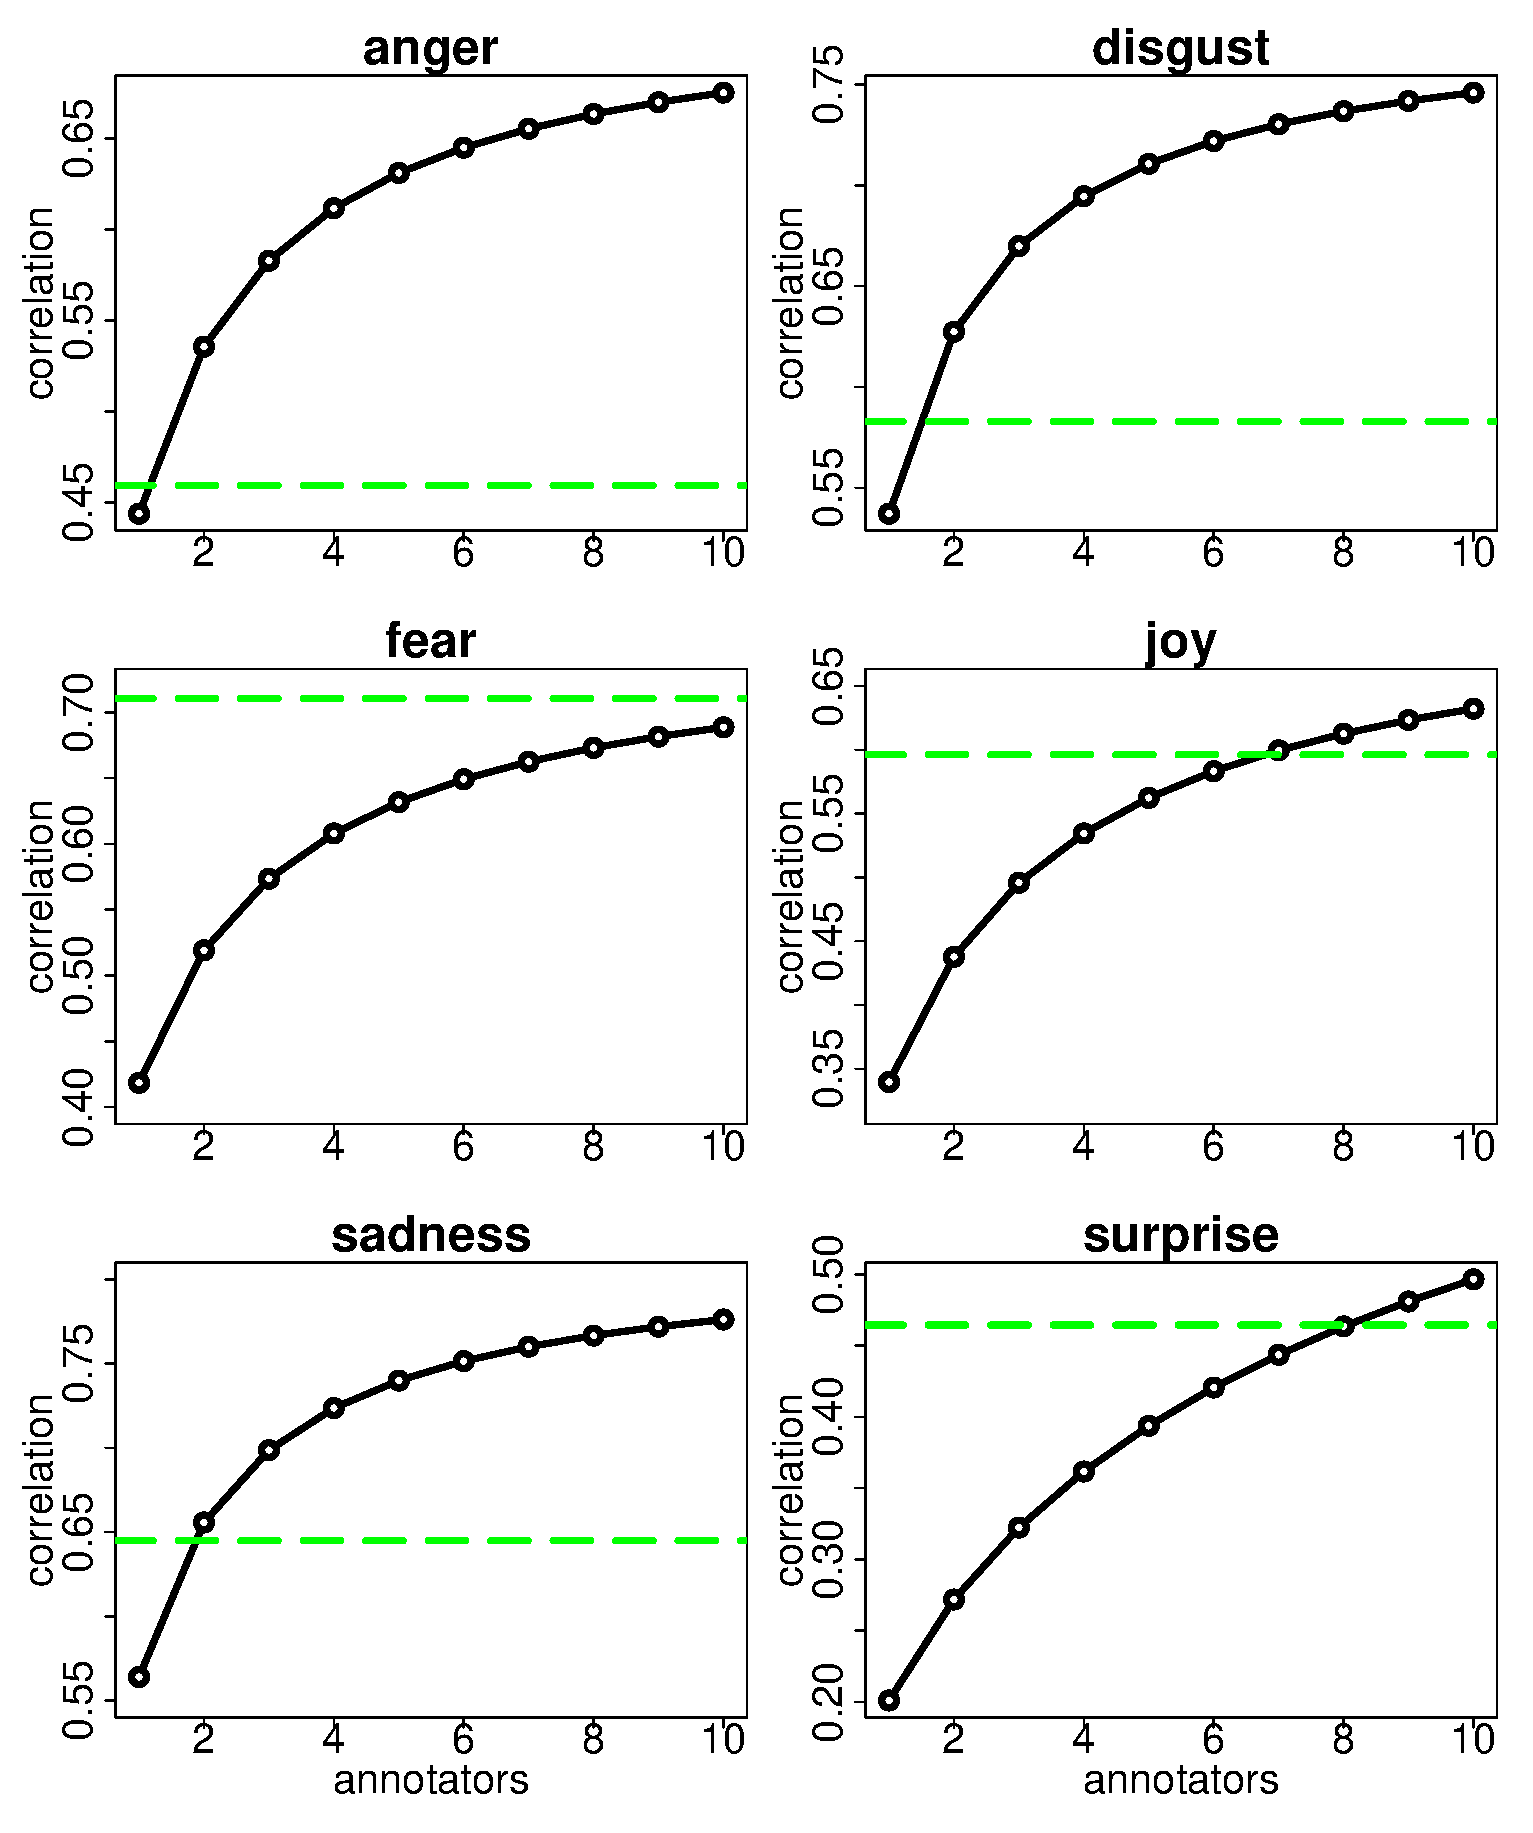
\includegraphics[width=8cm]{figures/all_emo.eps}
\caption{Sample affective text annotation} \label{affITAfigure}
\end{figure}

%Total annotations:  7000
%Total time: 5.93 hours
%Total cost:  \$2.00
%Avg anno / hour:  1180.4 anno /hour
%Avg anno / dollar: 3500 / 1 dollar
%Avg human-equiv labels / time:  
%Avg human-equiv labels / cost:  

\subsection{ Word Similarity }

This task replicates the word similarity task used in \cite{MC}, following a previous task initially proposed by \cite{RB}.  Specifically, we ask for numeric judgments of word similarity for 30 word pairs on a scale of [0,10], allowing fractional responses\footnote{\cite{MC} and others originally used a numerical score of [0,4].}  Numerous expert and non-expert studies have shown that this is task tends to yield very high interannotator agreement; \cite{MC} found a 0.97 correlation of the annotations of 38 subjects with the annotations given by 51 subjects in \cite{RG}, and a following study \cite{Resnik:99} with 10 subjects found a 0.96 correlation with \cite{MC}.

In our experiment we ask for 10 annotators, with each HIT containing the full 30 questions, at an offered price of \$0.02 / HIT; this task was completed in .  We evaluate our non-expert annotations by averaging the numeric responses from  each possible subset of $n$ non-expert annotations for each unit, for $n$ in the interval $[1,10]$.  We then treat this average as though it is the output of a single `meta-labeler', and compute the interannotator agreement with respect to the gold scores reported in \cite{MC}.  Our results are displayed in Figure \ref{wordsimITA}; at 10 annotators we achieve a correlation of 0.952, well within the range of other studies of experts and non-expert annotations.

\subsection{ Recognizing Textual Entailment }

This task replicates the recognizing textual entailment task originally proposed in \cite{rte1}; here the annotator is presented with two sentences
RTE 1
\cite{rte1}

RTE 3
\cite{rte3}
Also, we are able to do a further analysis of the results obtained in \cite{Zaenen:08}.

%\subsection{ Subjectivity Analysis? }
%Possible corpus: http://www.cs.pitt.edu/~wiebe/pubs/pub4.html
%MPQA Opinion Corpus annotated for opinions and sentiments

%\subsection{ Coreference Resolution? }
%Possible corpus:  MUC-6, MUC-7, ACE

\subsection{ Event Annotation}

This task is inspired by the temporal annotation corpus TimeBank \cite{TimeBank}.  This corpus consists of (X) sentences with Y labeled verb events;  these verb events have labeled with respect to neighboring verb events into one of six categories:  ()...

 [[ Explain the different even annotations:  before, after, overlapping, etc]]

We implement two simplified versions of this event annotation task:  in the simplest, we ask annotators to perform a forced binary choice on whether two verb events occur \textit{before} or \textit{after} one another, over the $N$ event pairs in TimeBank labeled with \textit{before} or \textit{after}.

Second, we give annotators the set of all labeled Timebank relations, and we ask for \textit{before}, \textit{after}, and \textit{other} labels.  Here we emphasize the notion of \textit{strictly before} and \textit{strictly after}.

[[ Task example ]]

\subsection{ Word Sense Disambiguation }

Here we annotate part of the Semeval Word Sense Disambiguation Lexical Sample task \cite{task17}; specifically, we annotate $N$ examples of the word president for the three senses given in Semeval.

[[ Task example ]]

%\subsection{ Machine Translation Evaluation?
%Possible corpus:  GALE HTER evaluations
%  better:  fluency / adequacy judgments.  another day...

\subsection{ Summary }

\begin{table}[h]
\footnotesize
    \begin{center}
        \begin{tabular}{|c||c|c|c|c|c|}
        \hline
        & & Cost & Time & Labels & Labels \\
        Task & Labels  & (USD) & (hrs) & per USD & per hr \\
        \hline
        Affect & 7000 & 2.0 & 5.93 & 3500 & 1180.4 \\
        WSim & 300 & 0.20 & 0.174 & 1500 & 1724.1 \\
        RTE & 1000 & 1.00 & 89.3 & 1000 & 11.20 \\
       % RTE3 &  &  & -- & -- \\
        Event & 4620 & 13.86 & 39.9 & 333.33 & 115.85 \\
        WSD & 1770 & 1.76 & 8.59 & 1005.7 & 206.1  \\
        \hline
        Total & 14690 & 18.82 & 143.87 & 780.55 & 102.11\\
        \hline
        \end{tabular}
    \caption{Summary of costs for non-expert labels}\label{costs}
\end{center}
\end{table}

In Table \ref{costs} we give a summary of the costs associated with obtaining the non-expert annotations for each of our 5 tasks.  Here \textit{time} is the given as the total amount of time elapsed from posing the request to AMT until the last assignment is submitted; it is not expected that workers are working on the task over the course of this time.


\section{ Bias correction for non-expert annotators  }

[[ just "bias" isn't quite everything.  maybe... ... bias and variance ... bias and noise ... bias and reweighting .... no, those are all too verbose ]]

The reliability of individual Turkers can vary greatly.  Some are move slowly and are more careful; some are more careless and make more mistakes; and a small few give very noisy responses.  Using a largery number of workers per example is very effective to control such noise, but we also explored several methods of correcting their biases.

[[ here is the case for bias correction: show a graph of individual worker accuracies.  or maybe the prolificness vs. accuracy scatterplot ]]

A wide number of methods have been explored to correct for the bias of annotators.

[[Here we could cite Dawid, Wiebe, Stork...  ]]

Here we consider the problem of using a small amount of expert-labeled training data in order to correct for the individual biases of different non-expert annotators.  For both categorical and numeric labels, rescale individual responses, and also weight more reliable workers more heavily.

\subsection{ Bias correction in categorical data }

\subsubsection{ Global bias }

[[ umm actually maybe don't do a global bias section.  the thresholding trick doesnt work for any of these NLP data sets, i think because the priors are very balanced and overall worker performance is pretty good. ]]


\subsubsection{ Categorical worker model }

We model labels and workers with a multinomial model similar to Naive Bayes.
Every example $i$ has a true label $x_i$.  For simplicity, assume two labels $\{Y,N\}$.   Several different workers give labels $y_{i1}, y_{i2}, .. y_{iK}$.  For the entire data set there are workers $w \in \{1..W\}$ though only several $K$ annotate a single example.  Each worker's judgment is conditionally independent of other workers.  A worker's condtional probability of response is modeled as multinomial.

To infer the posterior probability of the true label for a new example, worker judgments are integrated via Bayes rule and the conditional independence assumption:

\begin{eqnarray*}
&& \log \frac{P(x_i = Y  | y_{i1} .. y_{iW}) }{ P(x_i=N | y_{i1} .. y_{iW})  }  \\
&=& \sum_w \log \frac{ P(y_{iw} | x_i = Y) }{ P(y_{iw} | x_i = N) } + \log \frac{P(x_i=Y)}{P(x_i=N)} \\
\end{eqnarray*}

The worker response likelihoods $P(y_w | x=Y)$ and $P(y_w | x=N)$ can be directly estimated from frequencies of worker performance on gold standard examples.  (With 0 pseudocounts, each $y_w | x$ is just each worker's empirical confusion matrix.)  For MAP label estimation, the above equation describes a weighted voting rule: each Turker's vote is weighted by their log likelihood ratio for their given response.  Intuitively, workers who are more than 50\% accurate have positive votes; workers whose judgments are pure noise have zero votes; workers whose labels are anticorrelated have negative votes.

\subsubsection{ Example task: RTE-1 }

[[ experimental setup: leave one out cross-validation.  todo need results for varying the gold size.  worker label pseudoconts=1/2 or whatever they are.  example label priors are uniform, which is close to empirical.  or use empirical rates if its more accurate ]]

Figure \ref{RTEWorkers} shows improved accuracy at different numbers of annotators.  The lowest line is for the naive 50\% majority voting rule.  (This is equivalent to the above model with uniform priors and equal accuracies across workers and labels.)

[[ rion, did you already explain the subsampling further up?  probably dont have to talk about the worker sampling method? ]]

The modeling is most useful at low numbers of annotators, because a single biased or noisy worker can have a greater impact.

[[ maybe have line for accuracy-only model (constrained multinomial, only have diagonal vs nondiagonal rates) .  it's easier to explain; intuitive explanations of the model use "accuracy per worker" terminology anyway.  ]]

[[ (EM requires more trickiness for priors, but probably will skip it...?) ]]


\begin{figure}[ht]
\centering
%\includegraphics[width=8cm]{figures/calibration_example.eps}
\caption{Sample RTE calibration [[brendan todo: much better graph} \label{RTEWorkers}
\end{figure}

\subsection{ Bias correction for numeric data }

[[ we might expect numeric data to be especially prone to different workers having different judgment scales and such.  since we're averaging across workers, makes especial sense to recalibrate against the gold.  do graphs ehre?  they illustrate the point.  or maybe wait for the "Example task" section. ]]


\subsubsection{ Worker model }

[[ backslash R doesnt work i dont remember the tex for this ]]

Examples $i$ have true numeric labels $x_i$ all sharing the same prior distribution $N(\mu_x, \sigma_x)$.  Workers give responses $y_{iw} \in R$.  We explored several models of worker response.  The first is that each worker takes the original signal and adds their own bias and Gaussian noise:

\[ y_w | x \sim N( x + b_w, \sigma_w^2) \]

Given several worker responses, the MAP estimate of a label is
\begin{eqnarray*}
&& \arg\max_x \log p(x | y_1 .. y_K) \\
& =& \arg\max_x \sum_w \log p(y_w|x) + \log p(x) \\
& =& \arg\max_x \sum_w -\frac{1}{2\sigma_w^2} (x - (y_w - b))^2  + \\ && -\frac{1}{2\sigma_x^2} (x - \mu_x)^2
\end{eqnarray*}

The MAP solution for $x$ is the weighted mean of $y_w-b$, with weights $1/\sigma_w^2$, including the prior $\mu_x$ and weight $1/\sigma_x^2$ as well.

The second model is an ordinary linear model:  [[ this is "ordinary" in the sense of "OLS", right? ]]

\[ y_w | x \sim N( a_w x + b_w, \sigma_w^2 ) \]

With the MAP estimate being the weighted mean of $(y_w - b)/a$, weighted by $a^2/\sigma_w^2$ (plus the prior).
 
[[ and a third coming if it works out ]]

\subsubsection{ Example task:  Emotion annotation }

[[ We used the previous models to calibrate judgments on the affect data set. ]]

[[ worker model graph: some per-worker scatterplots with constant and linear models drawn inside.  maybe just maybe correction arrows if they dont look too bad ]]

[[ and the \#anno vs pearson correlation graph again? ]]


\subsection{ Evaluation and Discussion }

Over the set of experiments we perform, we find that we are able to achieve an equivalent inter-annotator agreement averaging over no more than an average of (X) annotators;  this figure is lowered to (Y) using bias-corrected judgments. 

\section{ Training a classifier with volunteer annotations }

In this section we compare a simple classification system for the affect recognition task trained with expert and non-expert annotations.  

\subsection{ Experimental Design }


For the purpose of this experiment we create a simple bag-of-words unigram model for predicting affect and valence.  Our model is very similar to the SWAT system \cite{SWAT}, one of the top-performing systems on the SemEval Affective Text task. For each token $t$ that appears in our training set, we assign it a weight for each emotion $e$ equal to the average emotion score observed in each headline $H$ it participates in. i.e.,:

\begin{equation*}
Score(e,t) = \sum_{ \forall H: t \in H } Score(e,H)
\end{equation*}

Then we compute the score for an emotion $e$ of a new headline $H$ as the average score of the set of tokens we've observed in the training set (ignoring those tokens not in the training set) as:

\begin{equation*}
Score(e,H) = \sum_{ t \in H} \frac{ Score(e,t) }{ | H |}
\end{equation*}

Where $|H|$ is simply the number of tokens in headline $H$, ignoring tokens not observed in the training set.  Unlike the SWAT system we perform no lemmatization, synonym expansion, or any other preprocessing of the tokens;  we simply use whitespace-separated tokens within each headline.

We train on examples 500-599 from the original test set of Semeval Task 8, and test on the remaining 900 examples.  In order to compare between expert and non-expert trained classifiers we average performance over all sets of For each 

\subsection{ Experiments }

First we verify that our model gives reasonable performance on the full task, trained and evaluated on the gold standard labels:

Next we compare the performance of this model as trained on the annotations of volunteer annotations vs. the individual expert annotations.  Since we are fortunate to have the six separate expert annotations in this task, we can perform an extended systematic comparison of the performance of the classifier trained with expert vs. non-expert data.

For this evaluation we would like to compare the performance of a system trained on non-expert annotations to that one of one trained with expert annotations; in order to do this, we propose the following experiment:  for each expert annotator we train a system using only the judgments provided by that annotator, and then create a gold standard test set using the average of the responses of the remaining five labelers on that set.  In this way we create six systems and compute the average ...

\begin{table}[h]
\footnotesize
    \begin{center}
        \begin{tabular}{|c||c|c|c|c|}
        \hline
        Emotion & Exp & 10-NE & K & K-NE \\
        \hline
        Anger & 0.084 & 0.233 & 1 & 0.172 \\
        Disgust & 0.130 & 0.231 & 1 & 0.185 \\
        Fear & 0.159 & 0.247 & 1 & 0.176 \\
        Joy & 0.130 & 0.125 & -- & -- \\
        Sadness & 0.127 & 0.174 & 1 & 0.141 \\
        Surprise & 0.060 & 0.101 & 1 & 0.061 \\
        Valence & 0.159 & 0.229 & 2 & 0.146 \\
        \hline
        Avg. Emo & 0.116 & 0.185 & 1 & 0.135 \\
        Avg. All & 0.122 & 0.191 & 1 & 0.137 \\
        \hline
        \end{tabular}
    \caption{Performance comparison of expert-trained and non-expert-trained classifier on test-set}\label{affectSWAT}
\end{center}
\end{table}

Next we train systems using sets of non-expert annotator responses.  We train an individual system from each possible subset of $n$ annotators, for $n$ in the interval $[1,10]$.  We then test teach system using the six gold standards used in the expert annotations, and average across these.  We then average the results of these studies across each subset size; the result of this experiment are given in Table \ref{affectSWAT} and in figure [[figure]].

Surprisingly we find that for five of the seven tasks, the average system trained with a single set of non-expert annotations outperforms the average system trained the labels from a single expert.  One possible hypothesis for the cause of this non-intuitive result is that individual labelers tend to have a strong bias, and since multiple non-expert labelers may contribute to a single set of non-expert annotations, the annotator diversity may have the effect of reducing annotator bias.

\section{Conclusion}

We demonstrate the effectiveness of using Amazon Mechanical Turk for a wide variety of natural language annotation tasks.  We perform an in-depth evaluation of labeler data vs. expert annotations for six tasks; we discover that only a small number of annotations per unit are necessary in order to emulate the same performance as an expert annotator.  For our tasks, we find the average number of annotations necessary to emulate an expert is X, or Y with bias-correction.  This corresponds to X cents per question, (or Y cents with bias-correction).

%\subsection*{Acknowledgments}
%Thanks to Marie-Catherine de Marneffe, Mona Diab, Christiane Fellbaum, Thad Hughes, and Benjamin Packer for useful discussions.  Rion Snow is supported by an NSF Fellowship.  This work was supported in part by the Disruptive Technology Office (DTO)'s Advanced Question Answering for Intelligence (AQUAINT) Phase III Program.

\bibliographystyle{acl}
\begin{thebibliography}{}%\denselist

%@inproceedings{1034721,
% author = {Janyce M. Wiebe and Rebecca F. Bruce and Thomas P. O'Hara},
% title = {Development and use of a gold-standard data set for subjectivity classifications},
% booktitle = {Proceedings of the 37th annual meeting of the Association for Computational Linguistics on Computational Linguistics},
% year = {1999},
% isbn = {1-55860-609-3},
% pages = {246--253},
% location = {College Park, Maryland},
% doi = {http://dx.doi.org/10.3115/1034678.1034721},
% publisher = {Association for Computational Linguistics},
% address = {Morristown, NJ, USA},
% }

\bibitem[\protect\citename{Baker et al.}1998]{FrameNet}
Collin F. Baker, Charles J. Fillmore, and John B. Lowe.
\newblock 1998.
\newblock The Berkeley FrameNet project. 
\newblock In \textit{Proc. of COLING-ACL 1998}.

\bibitem[\protect\citename{Chklovski and Mihalcea}2002]{WordExpert}
Timothy Chklovski and Rada Mihalcea.
\newblock 2002.
\newblock Building a sense tagged corpus with Open Mind Word Expert. 
\newblock In \textit{ Proc. of the Workshop on "Word Sense Disambiguation: Recent Successes and Future Directions", ACL 2002}.

\bibitem[\protect\citename{Chklovski and Gil}2005]{Chklovski:05}
Timothy Chklovski and Yolanda Gil.
\newblock 2005.
\newblock Towards Managing Knowledge Collection from Volunteer Contributors.
\newblock Proceedings of AAAI Spring Symposium on Knowledge Collection from Volunteer Contributors (KCVC05).

%\bibitem[\protect\citename{Chklovski and Mihalcea}2003]{Chklovski:03}
%Timothy Chklovski and Rada Mihalcea.
%\newblock 2003.
%\newblock Exploiting Agreement and Disagreement of Human Annotators for Word Sense Disambiguation.
%\newblock In {\it Proceedings of RANLP 2003}.

\bibitem[\protect\citename{Dagan et al.}2006]{rte1}
Ido Dagan, Oren Glickman and Bernardo Magnini. 
\newblock 2006.
\newblock The PASCAL Recognising Textual Entailment Challenge. 
\newblock Machine Learning Challenges. Lecture Notes in Computer Science, Vol. 3944, pp. 177-190, Springer, 2006.

\bibitem[\protect\citename{Dakka and Ipeirotis}2008]{Dakka:08}
Wisam Dakka and Panagiotis G. Ipeirotis.
\newblock 2008.
\newblock Automatic Extraction of Useful Facet Terms from Text Documents.
\newblock In \textit{Proc. of ICDE-2008}.

\bibitem[\protect\citename{Dawid and Skene}2008]{Dawid:79}
A. P. Dawid and A. M. Skene.
\newblock 2008.
\newblock Maximum Likelihood Estimation of Observer Error-Rates Using the EM Algorithm.
\newblock Applied Statistics, Vol. 28, No. 1 (1979), pp. 20-28.

%
%Christiane Fellbaum.
%\newblock 1998.
%\newblock WordNet: An Electronic Lexical Database.
%\newblock Cambridge, MA: MIT Press.

\bibitem[\protect\citename{Giampiccolo et al.}2007]{rte3}
Danilo Giampiccolo, Bernardo Magnini, Ido Dagan, and Bill Dolan.
\newblock 2007.
\newblock The third PASCAL recognizing textual entailment challenge.
\newblock In \textit{ Proc. of Workshop on Textual Entailment and Paraphrasing, ACL-2007}.

\bibitem[\protect\citename{Liu and Singh}2003]{ConceptNet}
Hugo Liu and Push Singh.
\newblock 2003.
\newblock ConceptNet: A practical commonsense reasoning toolkit.
\newblock BT Technology Journal, 22(4):211-226.

\bibitem[\protect\citename{Kaisser and Lowe}2008]{Kaisser:08a}
Michael Kaisser and John B. Lowe. 
\newblock 2008.
\newblock A Research Collection of Question�Answer Sentence Pairs.
\newblock In \textit{Proc. of LREC-2008}.

\bibitem[\protect\citename{Kaisser et al.}2008]{Kaisser:08b}
Michael Kaisser, Marti Hearst, and John B. Lowe. 
\newblock 2008.
\newblock Evidence for Varying Search Results Summary Lengths. 
\newblock In \textit{Proc. of ACL-2008}.

\bibitem[\protect\citename{Katz et al.}2007]{SWAT}
Phil Katz, Matthew Singleton, Richard Wicentowski. 
\newblock 2007.
\newblock SWAT-MP: The SemEval-2007 Systems for Task 5 and Task 14.
\newblock In \textit{ Proc. of SemEval-2007}.

\bibitem[\protect\citename{Kittur et al.}2008]{Kittur:08}
Aniket Kittur, Ed H. Chi, and Bongwon Suh. 
\newblock 2008.
\newblock Crowdsourcing user studies with Mechanical Turk. 
\newblock In \textit{ Proc. of CHI-2008}.

\bibitem[\protect\citename{Marcus et al.} 1993]{TreeBank}
Mitchell P. Marcus , Mary Ann Marcinkiewicz , and Beatrice Santorini.
\newblock 1993.
\newblock Building a large annotated corpus of English: the Penn Treebank.
\newblock Computational Linguistics, v.19 n.2, June 1993.

\bibitem[\protect\citename{Miller and Charles} 1991]{Miller:91}
George A. Miller and William G. Charles.
\newblock 1991.
\newblock Contextual Correlates of Semantic Similarity.
\newblock Language and Cognitive Processes, vol. 6, no. 1, pp. 1-28, 1991.

\bibitem[\protect\citename{Miller et al.} 1993]{SemCor}
George A. Miller, Claudia Leacock, Randee Tengi, and Ross T. Bunke.
\newblock 1993.
\newblock A semantic concordance.
\newblock In \textit{Proc. of HLT-1993}.

\bibitem[\protect\citename{Nakov}2008]{Nakov:08}
Preslav Nakov.
\newblock 2008.
\newblock Paraphrasing Verbs for Noun Compound Interpretation.
\newblock In \textit{Proc. of the Workshop on Multiword Expressions, LREC-2008}.

\bibitem[\protect\citename{Palmer et al.}2005]{PropBank}
Martha Palmer, Dan Gildea, and Paul Kingsbury.
\newblock 2005.
\newblock The Proposition Bank: A Corpus Annotated with Semantic Roles.
\newblock Computational Linguistics Journal, 31:1, 2005.

\bibitem[\protect\citename{Pradhan et al.} 2007]{task17}
Sameer Pradhan, Edward Loper, Dmitriy Dligach and Martha Palmer. 
\newblock 2007.
\newblock SemEval-2007 Task-17: English Lexical Sample, SRL and All Words. 
\newblock In \textit{ Proc. of the Fourth International Workshop on Semantic Evaluations (SemEval-2007), Association for Computational Linguistics, 2007}.

\bibitem[\protect\citename{Pustejovsky et al.}2003]{TimeBank}
James Pustejovsky, Patrick Hanks, Roser Saur�, Andrew See, Robert Gaizauskas, Andrea Setzer, Dragomir Radev, Beth Sundheim, David Day, Lisa Ferro and Marcia Lazo.
\newblock 2003.
\newblock The TIMEBANK Corpus. 
\newblock In \textit{Proc. of Corpus Linguistics 2003, 647-656.}

\bibitem[\protect\citename{Resnik}1999]{Resnik:99}
Philip Resnik. 
\newblock 1999.
\newblock Semantic Similarity in a Taxonomy: An Information-Based Measure and its Application to Problems of Ambiguity in Natural Language.
\newblock In JAIR, Volume 11, pages 95-130.

\bibitem[\protect\citename{Singh}2002]{OpenMindCommonSense}
Push Singh.
\newblock 2002. 
\newblock The public acquisition of commonsense knowledge.
\newblock In \textit{Proc. of AAAI Spring Symposium on Acquiring (and Using) Linguistic (and World) Knowledge for Information Access, 2002.}

\bibitem[\protect\citename{Stork}1999]{OpenMind}
David G. Stork.
\newblock 1999. 
\newblock The Open Mind Initiative.
\newblock IEEE Expert Systems and Their Applications pp. 16-20, May/June 1999.

\bibitem[\protect\citename{Strapparava and Mihalcea}2007]{AffectiveText}
Carlo Strapparava and Rada Mihalcea.
\newblock 2007.
\newblock SemEval-2007 Task 14: Affective Text
\newblock In \textit{Proc. of SemEval 2007}.

\bibitem[\protect\citename{Su et al.}2007]{Su:07}
Qi Su, Dmitry Pavlov, Jyh-Herng Chow, and Wendell C. Baker.
\newblock 2007.
\newblock Internet-Scale Collection of Human-Reviewed Data. 
\newblock In \textit{Proc. of WWW-2007}.

\bibitem[\protect\citename{von Ahn and Dabbish}2004]{espgame}
Luis von Ahn and Laura Dabbish.
\newblock 2004.
\newblock Labeling Images with a Computer Game.
\newblock In ACM Conference on Human Factors in Computing Systems, CHI 2004. Pages 319-326. 

\bibitem[\protect\citename{von Ahn et al.}2006]{verbosity}
Luis von Ahn, Mihir Kedia and Manuel Blum. 
\newblock 2006.
\newblock Verbosity: A Game for Collecting Common-Sense Knowledge. 
\newblock In ACM Conference on Human Factors in Computing Systems, CHI Notes 2006. Pages 75-78. 

\bibitem[\protect\citename{Voorhees and Dang}2006]{Voorhees:06}
Ellen Voorhees and Hoa Trang Dang.
\newblock 2006.
\newblock Overview of the TREC 2005 question answering track.
\newblock In \textit{ Proc. of TREC-2005}.

\bibitem[\protect\citename{Zaenen}2008]{Zaenen:08}
Annie Zaenen. 
\newblock Submitted.
\newblock Do give a penny for their thoughts.
\newblock International Journal of Natural Language Engineering (submitted).

\end{thebibliography}

\end{document}
